\documentclass{exam-zh}
\usepackage{edu-practice}

\examsetup{
  question/show-answer = true,
  fillin/show-answer = true,
  solution/show-solution = show-stay,
}

% ---------- 教师版解答样式 ----------
\newtcolorbox{solutionblock}{
  enhanced, breakable,
  colback=edu-blue-bg,
  colframe=edu-blue!25,
  boxrule=0pt,
  borderline west={2pt}{0pt}{edu-blue!50},
  arc=0pt,
  left=3mm, right=3mm, top=2mm, bottom=2mm,
  before skip=2mm,
  after skip=3mm,
  fontupper=\small,
}

% 解答步骤编号
\newcounter{solstep}
\newcommand{\solstep}[2]{%
  \stepcounter{solstep}%
  \par\medskip
  \noindent\hangindent=6mm
  {\color{edu-blue}\bfseries\textcircled{\scriptsize\thesolstep}\enspace #1}\enspace #2\par
}

\begin{document}

\section*{黄金分割比专项作业（教师版）}

\section*{黄金分割比专项 · 第 1 题}

\needspace{8\baselineskip}

\begin{problem}[points=8]
  \noindent
  \begin{minipage}[t]{\dimexpr\linewidth-42mm-6mm\relax}
    \vspace{0pt}
    在自然观察手账中，同学想画一朵向日葵花盘的径向示意线。花心到花瓣外缘长 $20\text{ cm}$，为了让花瓣环的位置看起来更接近自然花序的疏密美感，准备让花瓣环成为这条径向线的黄金分割点，并且从花心到花瓣环为较长一段。求从花心到花瓣环的长度。

    
  \end{minipage}\hfill
  \begin{diagramcoltikz}{42mm}{花盘径向线}
  
\includegraphics[width=\linewidth]{\detokenize{images/gr1-sunflower.png}}
  \end{diagramcoltikz}
  \par\medskip
  \setcounter{solstep}{0}
  \begin{solutionblock}
    \textbf{答案：}$10(\sqrt5-1)\text{ cm}$\par\medskip
    \solstep{列式}{$20\times\dfrac{\sqrt5-1}{2}=10(\sqrt5-1)\text{ cm}$。}
  \end{solutionblock}
\end{problem}


\clearpage
\section*{黄金分割比专项 · 第 2 题}

\needspace{8\baselineskip}

\begin{problem}[points=8]
  \noindent
  \begin{minipage}[t]{\dimexpr\linewidth-42mm-6mm\relax}
    \vspace{0pt}
    设计一张带传统纹样的书签时，较长的纹样区用来放莲花纹，长 $15\text{ cm}$；较短的留白区用来写姓名。为了让纹样和留白有更舒服的比例，设计师让较短留白区和较长纹样区成黄金分割比。求较短留白区的长度。

    
  \end{minipage}\hfill
  \begin{diagramcoltikz}{42mm}{书签分区}
  
\includegraphics[width=\linewidth]{\detokenize{images/gr2-bookmark.png}}
  \end{diagramcoltikz}
  \par\medskip
  \setcounter{solstep}{0}
  \begin{solutionblock}
    \textbf{答案：}$\dfrac{15(\sqrt5-1)}{2}\text{ cm}$\par\medskip
    \solstep{列式}{$15\times\dfrac{\sqrt5-1}{2}=\dfrac{15(\sqrt5-1)}{2}\text{ cm}$。}
  \end{solutionblock}
\end{problem}


\clearpage
\section*{黄金分割比专项 · 第 3 题}

\needspace{8\baselineskip}

\begin{problem}[points=8]
  \noindent
  \begin{minipage}[t]{\dimexpr\linewidth-42mm-6mm\relax}
    \vspace{0pt}
    舞蹈舞台的背景幕布上有一条横向光带，导演把它分成“静区”和“亮区”两段，让演员站位偏在黄金分割附近。较短的静区长 $6\text{ m}$，并且静区和较长的亮区成黄金分割比。求较长的亮区长度。

    
  \end{minipage}\hfill
  \begin{diagramcoltikz}{42mm}{舞台光带}
  
\includegraphics[width=\linewidth]{\detokenize{images/gr3-stage.png}}
  \end{diagramcoltikz}
  \par\medskip
  \setcounter{solstep}{0}
  \begin{solutionblock}
    \textbf{答案：}$3(\sqrt5+1)\text{ m}$\par\medskip
    \solstep{列式}{$6\div\dfrac{\sqrt5-1}{2}=3(\sqrt5+1)\text{ m}$。}
  \end{solutionblock}
\end{problem}


\clearpage
\section*{黄金分割比专项 · 第 4 题}

\needspace{8\baselineskip}

\begin{problem}[points=8]
  \noindent
  \begin{minipage}[t]{\dimexpr\linewidth-42mm-6mm\relax}
    \vspace{0pt}
    园林里一条总长 $34\text{ m}$ 的赏花小径，常把观景点放在不正中、但看起来很自然的位置。园艺师准备让观景点成为这条小径的黄金分割点，并且从入口到观景点为较短一段。求从入口到观景点的长度。

    
  \end{minipage}\hfill
  \begin{diagramcoltikz}{42mm}{赏花小径}
  
\includegraphics[width=\linewidth]{\detokenize{images/gr4-garden.png}}
  \end{diagramcoltikz}
  \par\medskip
  \setcounter{solstep}{0}
  \begin{solutionblock}
    \textbf{答案：}$17(3-\sqrt5)\text{ m}$\par\medskip
    \solstep{列式}{$34\times\dfrac{3-\sqrt5}{2}=17(3-\sqrt5)\text{ m}$。}
  \end{solutionblock}
\end{problem}


\clearpage
\section*{黄金分割比专项 · 第 5 题}

\needspace{8\baselineskip}

\begin{problem}[points=8]
  \noindent
  \begin{minipage}[t]{\dimexpr\linewidth-42mm-6mm\relax}
    \vspace{0pt}
    摄影构图时，摄影师常把主体放在画面黄金分割线附近，而不是正中间。一张照片裁切后，主体所在位置是这条边上的黄金分割点；主体到较远边的长留白为 $18\text{ cm}$，并且这段长留白是较长一段。求原来整条边的长度。

    
  \end{minipage}\hfill
  \begin{diagramcoltikz}{42mm}{摄影构图}
  
\includegraphics[width=\linewidth]{\detokenize{images/gr5-photo.png}}
  \end{diagramcoltikz}
  \par\medskip
  \setcounter{solstep}{0}
  \begin{solutionblock}
    \textbf{答案：}$9(\sqrt5+1)\text{ cm}$\par\medskip
    \solstep{列式}{$18\div\dfrac{\sqrt5-1}{2}=9(\sqrt5+1)\text{ cm}$。}
  \end{solutionblock}
\end{problem}


\clearpage
\section*{黄金分割比专项 · 第 6 题}

\needspace{8\baselineskip}

\begin{problem}[points=8]
  \noindent
  \begin{minipage}[t]{\dimexpr\linewidth-42mm-6mm\relax}
    \vspace{0pt}
    古典建筑立面常用黄金分割的比例安排窗格，让墙面不显得呆板。一段窗格被分成长短两段，其中较短窗格长 $4\text{ m}$，且较短窗格和较长窗格成黄金分割比。求整段窗格的长度。

    
  \end{minipage}\hfill
  \begin{diagramcoltikz}{42mm}{窗格分段}
  
\includegraphics[width=\linewidth]{\detokenize{images/gr6-architecture.png}}
  \end{diagramcoltikz}
  \par\medskip
  \setcounter{solstep}{0}
  \begin{solutionblock}
    \textbf{答案：}$(6+2\sqrt5)\text{ m}$\par\medskip
    \solstep{列式}{$4\div\dfrac{3-\sqrt5}{2}=(6+2\sqrt5)\text{ m}$。}
  \end{solutionblock}
\end{problem}


\clearpage
\section*{黄金分割比专项 · 第 7 题}

\needspace{8\baselineskip}

\begin{problem}[points=8]
    我们将宽和长之比为 $\dfrac{\sqrt5-1}{2}$（约为 $0.618$）的矩形称为“黄金矩形”，它可以通过折纸获得。

如图 1 所示，将长方形纸片第一次沿 $MC$ 折叠，使点 $N$ 和点 $B$ 重合；展开后再将纸片沿 $AG$ 对折，使点 $M$ 和点 $B$ 重合。如图 2 所示，展开后联结 $AB$，再将纸片第三次沿 $AF$ 折叠，使得 $AB$ 落在长方形纸片的边上且点 $B$ 落在点 $D$ 处；再次展开，过点 $D$ 作 $MB$ 的垂线，垂足为点 $E$。请写出图中的“黄金矩形”。

\begin{center}
  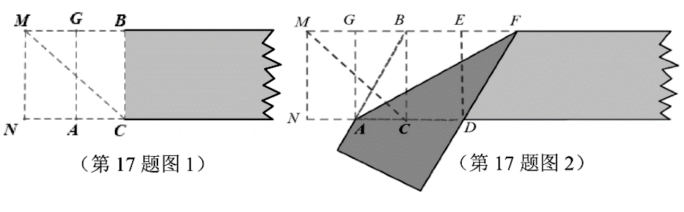
\includegraphics[width=0.92\linewidth]{images/golden-rectangle-folding-source.png}
\end{center}

    
  \setcounter{solstep}{0}
  \begin{solutionblock}
    \textbf{答案：}矩形 $BCDE$\par\medskip
    \solstep{解答}{由折叠得 $MB=BC$，$AC=\dfrac12BC$，$AB=AD=\dfrac{\sqrt5}{2}BC$，所以 $CD=AD-AC=\dfrac{\sqrt5-1}{2}BC$。又 $DE\perp MB$，故黄金矩形为矩形 $BCDE$。}
  \end{solutionblock}
\end{problem}


\clearpage
\section*{答案速查}


\begin{keyideabox}
  \textbf{答案}
  第1题 $10(\sqrt5-1)\text{ cm}$；第2题 $\dfrac{15(\sqrt5-1)}{2}\text{ cm}$；第3题 $3(\sqrt5+1)\text{ m}$；
第4题 $17(3-\sqrt5)\text{ m}$；第5题 $9(\sqrt5+1)\text{ cm}$；第6题 $(6+2\sqrt5)\text{ m}$；第7题 矩形 $BCDE$。

\end{keyideabox}



\end{document}
